\documentclass{standalone}
\usepackage{xparse}
\usepackage{tikz}
\tikzset{%
  point/.style={circle,inner sep=1.25pt,minimum size=1.25pt,draw,fill=#1},
  point/.default=red
}
\definecolor{c0}{rgb}{0.2,0.4,0.67}
\definecolor{c1}{rgb}{0.67,0.4,0.12}
\definecolor{c2}{rgb}{0.53,0.6,0.13}
\definecolor{c3}{rgb}{0.53,0.53,0.4}
\NewDocumentCommand\witness{mmmO{c2}}{%
  \node[point=#4] (w0) at (#1) {};
  \node[point=#4] (w1) at (#2) {};
  \node[point=#4] (w2) at (#3) {};
  \draw[#4] (w0)--(w1)--(w2);
}
\def\myWitness{\witness{0,0}{\x,\y}{\dc,0}}
\NewDocumentCommand\crvb{}{%
  \def\a{-0.618034}
  \def\b{-1.61803}
  \def\c{.52573}
  \def\s{.85065}
  \draw[c1,parametric,variable=\t,smooth,
    domain=1:2.6,
    samples=60]
  plot
  ({\a*cos(\t r)*\c-\b*sin(\t r)*\s},{\a*cos(\t r)*\s+\b*sin(\t r)*\c});
}
\begin{document}
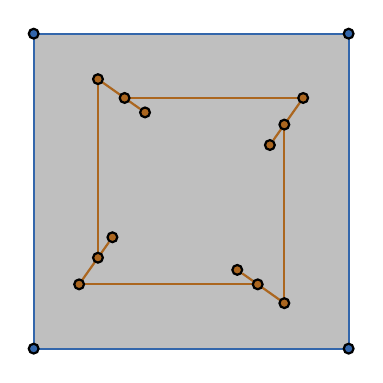
\begin{tikzpicture}[thick]
  % Boundary
  \coordinate (b0) at (-2,-2);
  \coordinate (b1) at (2,-2);
  \coordinate (b2) at (2,2);
  \coordinate (b3) at (-2,2);
  \filldraw[fill=lightgray,draw=c0] (b0) -- (b1) -- (b2) -- (b3) -- cycle;
  \node[point=c0] at (b0) {};
  \node[point=c0] at (b1) {};
  \node[point=c0] at (b2) {};
  \node[point=c0] at (b3) {};
  % Solution segments
  \pgfmathparse{1}\let\da\pgfmathresult
  \pgfmathparse{sqrt(2)}\let\db\pgfmathresult
  \pgfmathparse{pi*0.5}\let\angle\pgfmathresult
  \pgfmathparse{cos(deg(\angle))}\let\c\pgfmathresult
  \pgfmathparse{sqrt(\da*\da+\db*\db-2*\c*\da*\db)}\let\dc\pgfmathresult
  \pgfmathparse{(\dc*\dc-\db*\db+\da*\da)/(2*\dc)}\let\x\pgfmathresult
  \pgfmathparse{sqrt(\da*\da-\x*\x)}\let\y\pgfmathresult
  %
  \coordinate[shift={(-2,-2)}] (a0) at (\x,\y);
  \coordinate[shift={(2-\dc,-2)}] (a1) at (\x,\y);
  \begin{scope}[rotate=90,shift={(-2,-2)}]\coordinate (a2) at (\x,\y);\end{scope}
  \begin{scope}[rotate=90,shift={(2-\dc,-2)}]\coordinate (a3) at (\x,\y);\end{scope}
  \begin{scope}[rotate=180,shift={(-2,-2)}]\coordinate (a4) at (\x,\y);\end{scope}
  \begin{scope}[rotate=180,shift={(2-\dc,-2)}]\coordinate (a5) at (\x,\y);\end{scope}
  \begin{scope}[rotate=270,shift={(-2,-2)}]\coordinate (a6) at (\x,\y);\end{scope}
  \begin{scope}[rotate=270,shift={(2-\dc,-2)}]\coordinate (a7) at (\x,\y);\end{scope}
  \draw[c1] (a0)--(a1);
  \draw[c1] (a2)--(a3);
  \draw[c1] (a4)--(a5);
  \draw[c1] (a6)--(a7);
  \node[point=c1,shift={(-2,-2)}] (a8) at (\da,\db) {};
  \draw[c1] (a0)--(a8);
  \begin{scope}[rotate=90,shift={(-2,-2)}]\node[point=c1] (a9) at (\da,\db) {};\end{scope}
  \draw[c1] (a2)--(a9);
  \begin{scope}[rotate=180,shift={(-2,-2)}]\node[point=c1] (a10) at (\da,\db) {};\end{scope}
  \draw[c1] (a4)--(a10);
  \begin{scope}[rotate=270,shift={(-2,-2)}]\node[point=c1] (a11) at (\da,\db) {};\end{scope}
  \draw[c1] (a6)--(a11);
  % Witnesses
  \begin{scope}[shift={(-2,-2)}]\myWitness\end{scope}
  \begin{scope}[shift={(2-\dc,-2)}]\myWitness\end{scope}
  \begin{scope}[shift={(-2,-2+\dc)},rotate=270]\myWitness\end{scope}
  \begin{scope}[shift={(-2,-2+\db)},rotate=305]\myWitness\end{scope}
  %%
  %% \begin{scope}[shift={(1,-1)},rotate=270]\witness[p1][q1][r1][c2!20!black]\end{scope}
  %% \begin{scope}[shift={(1.06,-.721)},rotate=250]\witness[p2][q2][r2][c2!40!black]\end{scope}
  %% \begin{scope}[shift={(1.2929,-.5858)},rotate=225]\witness[p3][q3][r3][c2!60!black]\end{scope}
  %% \begin{scope}[shift={(1.655,-.717)},rotate=200]\witness[p4][q4][r4][c2!80!black]\end{scope}
  %% \begin{scope}[shift={(2,-1)},rotate=180]\witness[p5][q5][r5][c2!100!black]\end{scope}
  %% %%
  %% \begin{scope}[shift={(-2,2)},rotate=0]\crvb\end{scope}
  %% \begin{scope}[shift={(-2,-2)},rotate=90]\crvb\end{scope}
  %% \begin{scope}[shift={(2,-2)},rotate=180]\crvb\end{scope}
  %% \begin{scope}[shift={(2,2)},rotate=270]\crvb\end{scope}
  %% %%
  \node[point=c1] (n0) at (a0) {};
  \node[point=c1] (n1) at (a1) {};
  \node[point=c1] (n2) at (a2) {};
  \node[point=c1] (n3) at (a3) {};
  \node[point=c1] (n4) at (a4) {};
  \node[point=c1] (n5) at (a5) {};
  \node[point=c1] (n6) at (a6) {};
  \node[point=c1] (n7) at (a7) {};
\end{tikzpicture}

\end{document}
